\section{Functional Requirements}

\subsection{Mandatory Functional Requirements}
\begin{description}
\item[/FM010/ Create XML-Configuration file]\hfill\\ User is able to create/generate XML-Configuration file.
\item[/FM020/ Open and view XML-Configuration file]\hfill\\ User is able to open XML files, if the file created or generated using \app{}.
\item[/FM030/ Save XML-Configuration file]\hfill\\ User is able to edit and save the existed XML-Configuration files using \textbf{FM020} and \textbf{FM030} combined and just save the new XML-Configuration files using \textbf{FM010} and \textbf{FM030} combined.
\end{description}

\subsection{Facultative Functional Requirements}
\begin{description}
\item[/FF010/ Run Telesales batch]\hfill\\ User is able to start Telesales batch application just clicking ``Start''-button. \app{} runs the batch application for the current opened or created configuration passing the right parameters to the Telesales batch application.
\end{description}

\begin{figure}[h!]
\centering
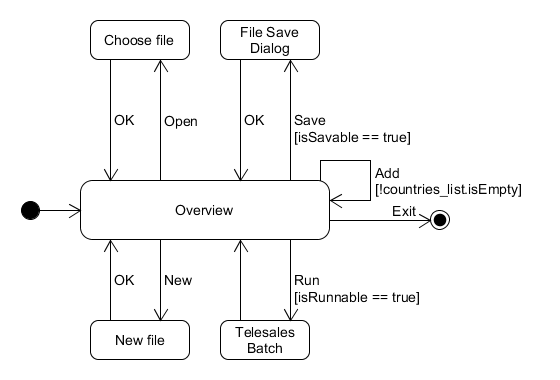
\includegraphics[width=\textwidth]{d_activity.png}
\caption{Activity diagram of the functional requirements}
\end{figure}
